\documentclass[tikz,border=1pt]{standalone}
\usepackage[T1]{fontenc}
\usepackage{lmodern}
\usetikzlibrary{arrows.meta}
\begin{document}
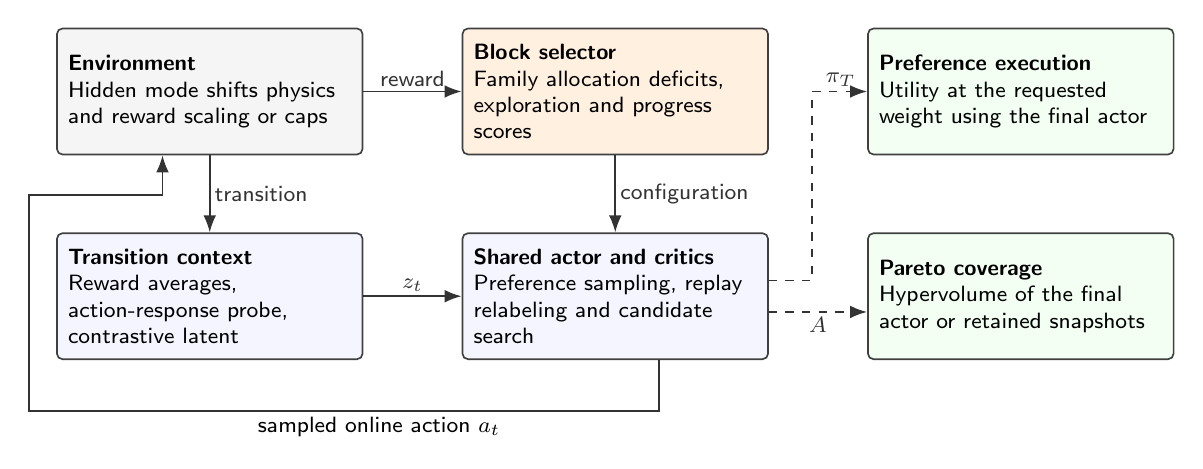
\begin{tikzpicture}[
    font=\sffamily\footnotesize,
    >=Latex,
    box/.style={
        draw=black!75, fill=#1, rounded corners=2pt, line width=.6pt,
        text width=36mm, minimum height=16mm,
        align=flush left, inner sep=4pt
    },
    arr/.style={->, line width=.7pt, color=black!80},
    eval/.style={arr,dashed},
    lbl/.style={inner sep=1.5pt}
]
\node[box=black!4] (env) at (0,2.6) {
    \textbf{Environment}\\
    Hidden mode shifts physics and reward scaling or caps
};
\node[box=blue!4] (ctx) at (0,0) {
    \textbf{Transition context}\\
    Reward averages, action-response probe, contrastive latent
};
\node[box=orange!12] (sel) at (5.15,2.6) {
    \textbf{Block selector}\\
    Family allocation deficits, exploration and progress scores
};
\node[box=blue!4] (ac) at (5.15,0) {
    \textbf{Shared actor and critics}\\
    Preference sampling, replay relabeling and candidate search
};
\node[box=green!5] (exec) at (10.3,2.6) {
    \textbf{Preference execution}\\
    Utility at the requested weight using the final actor
};
\node[box=green!5] (cov) at (10.3,0) {
    \textbf{Pareto coverage}\\
    Hypervolume of the final actor or retained snapshots
};
\draw[arr] (env.south) -- node[lbl,right] {transition} (ctx.north);
\draw[arr] (env.east) -- node[lbl,above] {reward} (sel.west);
\draw[arr] (ctx.east) -- node[lbl,above] {$z_t$} (ac.west);
\draw[arr] (sel.south) -- node[lbl,right] {configuration} (ac.north);
\draw[arr] ([xshift=0.55cm]ac.south) -- ++(0,-0.65)
    -| (-2.3,1.28) -| ([xshift=-0.6cm]env.south);
\node[lbl,below] at (2.15,-1.48) {sampled online action $a_t$};
\draw[eval] ([yshift=2mm]ac.east) -- ++(.55,0) |-
    node[lbl,above,pos=.76] {$\pi_T$} (exec.west);
\draw[eval] ([yshift=-2mm]ac.east) -- node[lbl,below] {$A$}
    ([yshift=-2mm]cov.west);
\end{tikzpicture}
\end{document}
